\section{\'Etude d'une épidémie (14 points)}\label{ex:epidemie}

Pendant une épidémie observée sur une période de onze jours, un institut de veille sanitaire a modélisé le nombre de personnes malades. La durée, écoulée à partir du début de la période et exprimée en jours, est notée $t$. Le nombre de cas, en fonction de la durée $t$ est est donné en milliers par la fonction $f$ de la variable réelle $t$ définie et dérivable sur l'intervalle $\left[0; 11\right]$, dont la représentation graphique $C_f$ est donnée en annexe \ref{app:fig}.

Cette annexe sur laquelle le candidat pourra faire figurer des traits de constructions utiles au raisonnement, est à rendre avec la copie.

\subsection{\'Etude graphique}\label{sec:A}

\emph{Pour cette partie, on se réfèrera à la courbe représentative $C_f$ de la fonction f.}

\begin{questions}
	\question[2] On considère que la situation est grave lorsque le nombre de cas est d'au moins \num{150000} malades. Pendant combien de jours complets cela arrive-t-il ?
	\begin{solution}
		On dépasse les \num{150000} malades pendant 6 jours complets.
	\end{solution}
	
	\question[2] La droite $(OA)$ est la tangente à la courbe $C_f$ au point d'abscisse 0, où A est le point de coordonnées $(10;\num{112.5})$. Déterminer $f'(0)$ où $f'$ représente ta fonction dérivée de la fonction $f$.\label{q:drv}
	\begin{solution}
		$f'(0)$ est le coefficient directeur de la tangente en 0, donc de $(OA)$.
		
		\begin{eqnarray*}
			f'(0) &=& \frac{y_A - y_O}{x_A - x_O} \\
			f'(0) &=& \frac{\num{112.5} - 0}{10 - 0} \\
			f'(0) &=& \frac{\num{112.5}}{10} \\
			f'(0) &=& \num{11.25}
		\end{eqnarray*}
	\end{solution}
	
	\question Le nombre $f'(t)$ représente la vitesse d'évolution de la maladie, $t$ jours après l'apparition des premier cas.
		\begin{parts}
			\part[2] Déterminer graphiquement le nombre maximal de malades sur la période de 11 jours observés et le moment où il est atteint. Que peut-on dire alors de la vitesse d'évolution de la maladie ?
			\begin{solution}
				Sur la période observée, il y a eu au maximum environ 253 malades, c'est arrivé dans le courant du huitième jour ($x=\num{7.5}$).
			\end{solution}
			
			\part[1] Déterminer graphiquement à quel moment de l'épidémie la maladie progresse le plus.
			\begin{solution}
				Le moment où la maladie progresse le plus est celui où la pente de la courbe est la plus importante, cela arrive durant le quatrième jour.
			\end{solution}
		\end{parts}
\end{questions}


\subsection{\'Etude théorique}

La fonction $f$ de la \ref{sec:A} est définie par :

	\begin{equation*}
		f(t) = -t^3 + \frac{21}{2} t^2 + \frac{45}{4}t
	\end{equation*}
	
\begin{questions}
	\question[2] recopier et compléter, à l'aide de la calculatrice, le tableau suivant :
	\begin{center}
		
	\begin{tabular}{|@{\ }l@{\ }|@{\ \ }c@{\ \ }|@{\ \ }c@{\ \ }|@{\ \ }c@{\ \ }|@{\ \ }c@{\ \ }|@{\ \ }c@{\ \ }|@{\ \ }c@{\ \ }|@{\ \ }c@{\ \ }|@{\ \ }c@{\ \ }|@{\ \ }c@{\ \ }|@{\ \ }c@{\ \ }|@{\ \ }c@{\ \ }|@{\ \ }c@{\ \ }|}
		\hline
		$t$    & 0 & 1 & 2 & 3 & 4 & 5 & 6           & 7 & 8 & 9 & 10 & 11 \\ \hline
		$f(t)$ &   &   &   &   &   &   & \num{229.5} &   &   &   &    &    \\ \hline
	\end{tabular}
	\end{center}

	\begin{solution}
		\begin{center}
			
			\begin{tabular}{|@{\ }l@{\ }|@{\ }c@{\ }|@{\ }c@{\ }|@{\ }c@{\ }|@{\ }c@{\ }|@{\ }c@{\ }|@{\ }c@{\ }|@{\ }c@{\ }|@{\ }c@{\ }|@{\ }c@{\ }|@{\ }c@{\ }|@{\ }c@{\ }|@{\ }c@{\ }|}
				\hline
				$t$    & 0 & 1 & 2 & 3 & 4 & 5 & 6           & 7 & 8 & 9 & 10 & 11 \\ \hline
				$f(t)$ & 0  & \num{20.75}  & \num{56.5}  & \num{101.25}  & \num{149}  & \num{193.75}  & \num{229.5} & \num{250.25}  & \num{250}  & \num{222.75}  &  \num{165.5}  &  \num{63.25}  \\ \hline
			\end{tabular}
		\end{center}
	\end{solution}

	\question[2] Calculer $f'(t)$ et vérifier que, pour tout $t$ de l'intervalle $\left[0; 11\right]$ :
		\begin{equation*}
			f'(t) = -3 \left(t + \frac{1}{2} \right) \left(t - \frac{15}{2} \right)
		\end{equation*}
		
		\begin{solution}
			Calcul de la fonction dérivée $f'(t)$ :
			
			\begin{eqnarray*}
				f'(t) &=& 3 \times -t^2 + 2 \times \frac{21}{2} t + \frac{45}{4} \\
				f'(t) &=& -3t^2 + 21 t + \frac{45}{4} \\
			\end{eqnarray*}
		
			Développement de la forme factorisée
			\begin{eqnarray*}
				-3 \left(t + \frac{1}{2} \right) \left(t - \frac{15}{2} \right) &=& -3 \left( t^2 - \frac{15}{2}t + \frac{1}{2}t - \frac{15}{4}\right) \\
				-3 \left(t + \frac{1}{2} \right) \left(t - \frac{15}{2} \right) &=& -3 \left( t^2 - \frac{14}{2}t - \frac{15}{4}\right) \\
				-3 \left(t + \frac{1}{2} \right) \left(t - \frac{15}{2} \right) &=&  -3t^2 + 3 \times 7t + \frac{3 \times 15}{4}  \\
				-3 \left(t + \frac{1}{2} \right) \left(t - \frac{15}{2} \right) &=& -3t^2 + 21t + \frac{45}{4} \\
			\end{eqnarray*}
			
			On a donc bien $f'(t) = -3 \left(t + \frac{1}{2} \right) \left(t - \frac{15}{2} \right)$.
		\end{solution}
		
	\question[2] \'Etudier le signe de $f'(t)$ sur l'intervalle $\left[0; 11\right]$. Cette réponse est-elle cohérente avec la courbe $C_f$ ? Expliquer.
	
	\begin{solution}
		\'Etude du signe de $(t + \frac{1}{2})$ et de $(t - \frac{15}{2})$
		
		\begin{multicols}{2}
			\begin{eqnarray*}
				t + \frac{1}{2} & \ge & 0 \\
				t & \ge & - \frac{1}{2} \\
			\end{eqnarray*}
		
			\begin{eqnarray*}
				t - \frac{15}{2} & \ge & 0 \\
				t & \ge & \frac{15}{2} \\
			\end{eqnarray*}
		\end{multicols}
	
		On a donc : \\
		\begin{center}
			\begin{tikzpicture}[scale=0.8]
				\tkzTabInit{$t$/1.5,$-3$/1.5,$(t + \frac{1}{2})$/1.5,$(t - \frac{15}{2})$/1.5,$f'(t)$/1.5}{$0$, $\frac{15}{2}$, $11$}
				\tkzTabLine { ,- ,  , -}
				\tkzTabLine { ,+ ,  , +}
				\tkzTabLine { ,- ,z , +}
				\tkzTabLine { ,+ ,z , -}
			\end{tikzpicture}
		\end{center}
		
		Sur l'intervalle $\left[0 ; \num{7.5} \right]$ la courbe en annexe est croissante et la dérivée positive. Sur $\left[\num{7.5} ; 11 \right]$ la courbe est décroissante et la dérivée négative. Cette réponse est donc cohérente avec la courbe.
	\end{solution} 
	
	\question[1] Retrouver la résultat de la question \ref{q:drv} de la partie \ref{sec:A}.
	
	\begin{solution}
		Calcul de $f'(0)$ :
		
		\begin{eqnarray*}
			f'(0) &=& -3 \times 0^2 + 21 \times 0 + \frac{45}{4} \\
			f'(0) &=& \frac{45}{4} \\
			f'(0) &=& \num{11.25} \\
		\end{eqnarray*}
	
		On retrouve bien la valeur de $f'(0)$ trouvée à la question \ref{q:drv} de la partie \ref{sec:A}.
	\end{solution}
\end{questions}